\documentclass[twocolumn,a4j]{jsarticle}
\setlength{\topmargin}{-20.4cm}
\setlength{\oddsidemargin}{-10.4mm}
\setlength{\evensidemargin}{-10.4mm}
\setlength{\textwidth}{18cm}
\setlength{\textheight}{26cm}

\usepackage[top=15truemm,bottom=20truemm,left=15truemm,right=15truemm]{geometry}
\usepackage[latin1]{inputenc}
\usepackage{amsmath}
\usepackage{amsfonts}
\usepackage{amssymb}
\usepackage[dvipdfmx]{graphicx}
\usepackage[dvipdfmx]{color}
\usepackage{listings}
\usepackage{listings,jvlisting}
\usepackage{geometry}
\usepackage{framed}
\usepackage{color}
\usepackage[dvipdfmx]{hyperref}
\usepackage{ascmac}
\usepackage{enumerate}
\usepackage{tabularx}
\usepackage{cancel}
\usepackage{scalefnt}

\renewcommand{\figurename}{Fig.}
\renewcommand{\tablename}{Table }

\lstset{
basicstyle={\ttfamily},
identifierstyle={\small},
commentstyle={\smallitshape},
keywordstyle={\small\bfseries},
ndkeywordstyle={\small},
stringstyle={\small\ttfamily},
frame={tb},
breaklines=true,
columns=[l]{fullflexible},
xrightmargin=0zw,
xleftmargin=3zw,
numberstyle={\scriptsize},
stepnumber=1,
numbersep=1zw,
lineskip=-0.5ex
}

\makeatletter
\def\@maketitle
{
\begin{center}
{\LARGE \@title \par}
\end{center}
\begin{flushright}
{\large 報告書 NO.09 - 2\quad\@date\quad\@author}
\end{flushright}
\par\vskip 1.5em
}
\makeatother

\setcounter{tocdepth}{3}

\author{来代 勝胤}
\title{令和3年度 1月 第2週 報告書 (追記)}
\date{2022/1/13}

\begin{document}
\columnseprule=0.1mm

\maketitle
\section*{報告内容}
\begin{enumerate}[1.]
    \item 進捗状況
    \item 校正装置と供試体のオフセット(作成中)
    \item テストデータの作成
    \item 実験結果とテストデータの比較
    \item 次週の予定
\end{enumerate}

\section{進捗状況}
評価実験の結果に軸の回転を考慮した補正値を用いて,正味出力電圧を算出したところ
そのプロットした図(Fig.1)に周期的な振動が見られた.
今週は,その原因と考えられる校正装置と供試体の軸のオフセットを考慮したテストデータを作成し
補正プログラムを適用した出力結果と実験結果の比較を行った.

\section{校正装置と実験装置の軸のオフセット}

以前の補正理論では,実験装置と校正装置の軸の回転によるズレに着目し補正を行った.
しかし,そこから算出された正味出力電圧は一定値を示すことはなく,周期的な振動を示すような結果(Fig.4)を示した.\par
ここで,校正装置と実験装置の軸にオフセット(Fig.5)があることがその要因の一つと考えられる.
このオフセットについては,人為的な装置の設置過程では無視することが不可能な誤差である.
したがって,オフセットを考慮したテストデータを作成しその結果を見ることで
正味出力電圧における周期的な振動の原因・影響の大きさを調べる.

\begin{figure}[htbp]
    \footnotesize
    \begin{center}
        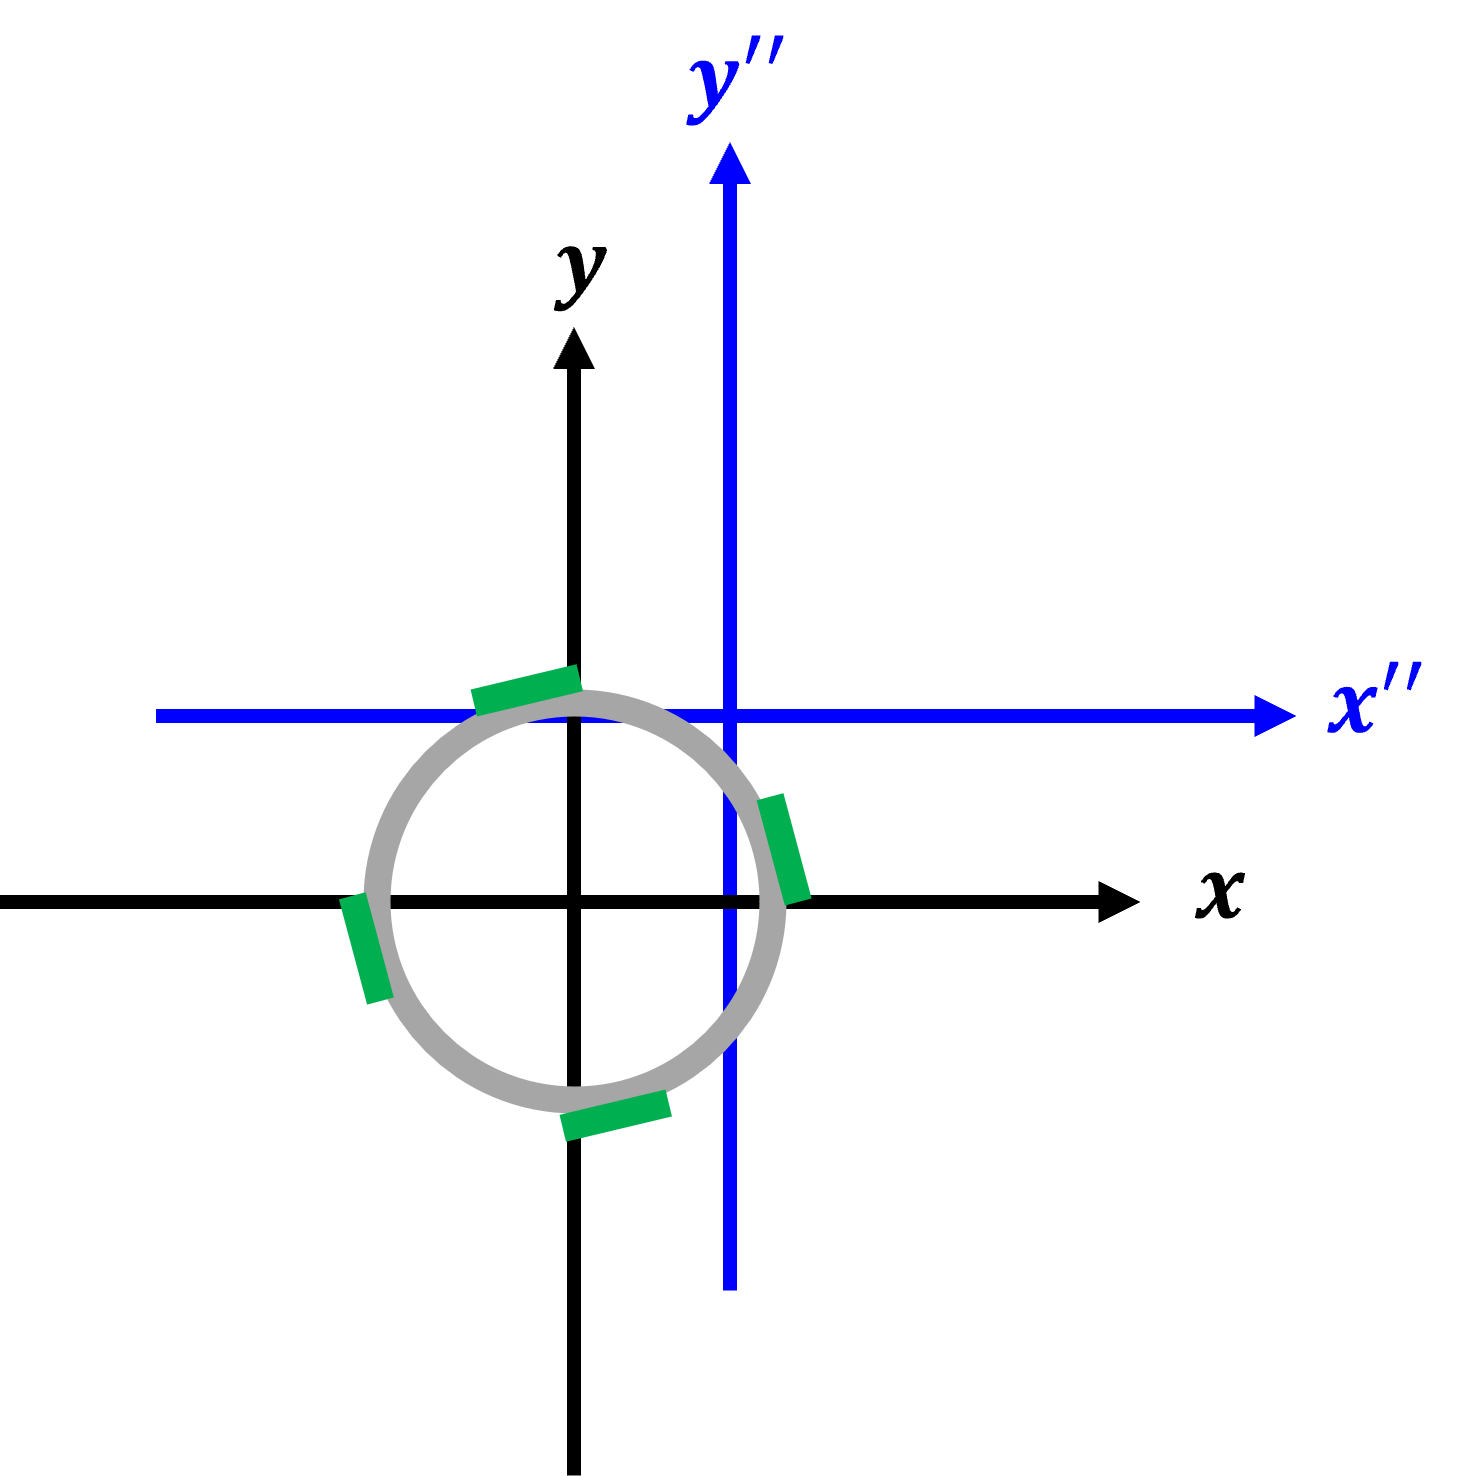
\includegraphics[width=65mm]{../images/image_5.png}
        \caption{}
    \end{center}
\end{figure}

\newpage

\subsection{オフセットによる出力電圧への影響}

はじめに,正規座標系$x-y$より,$\Delta x$,$\Delta y$だけ
移動した座標系$x''-y''$を校正装置における座標系とする.
ここで,供試体表面に任意の角度$\theta$から作用力$F$を加える.
このとき,作用力$F$は,$\Delta x$,$\Delta y$のオフセットを持つため,
座標系$x''-y''$の中心$o'$を通る.
すなわち,正規座標系における中心$o$を通ることはない.

\begin{figure}[htbp]
    \footnotesize
    \begin{center}
        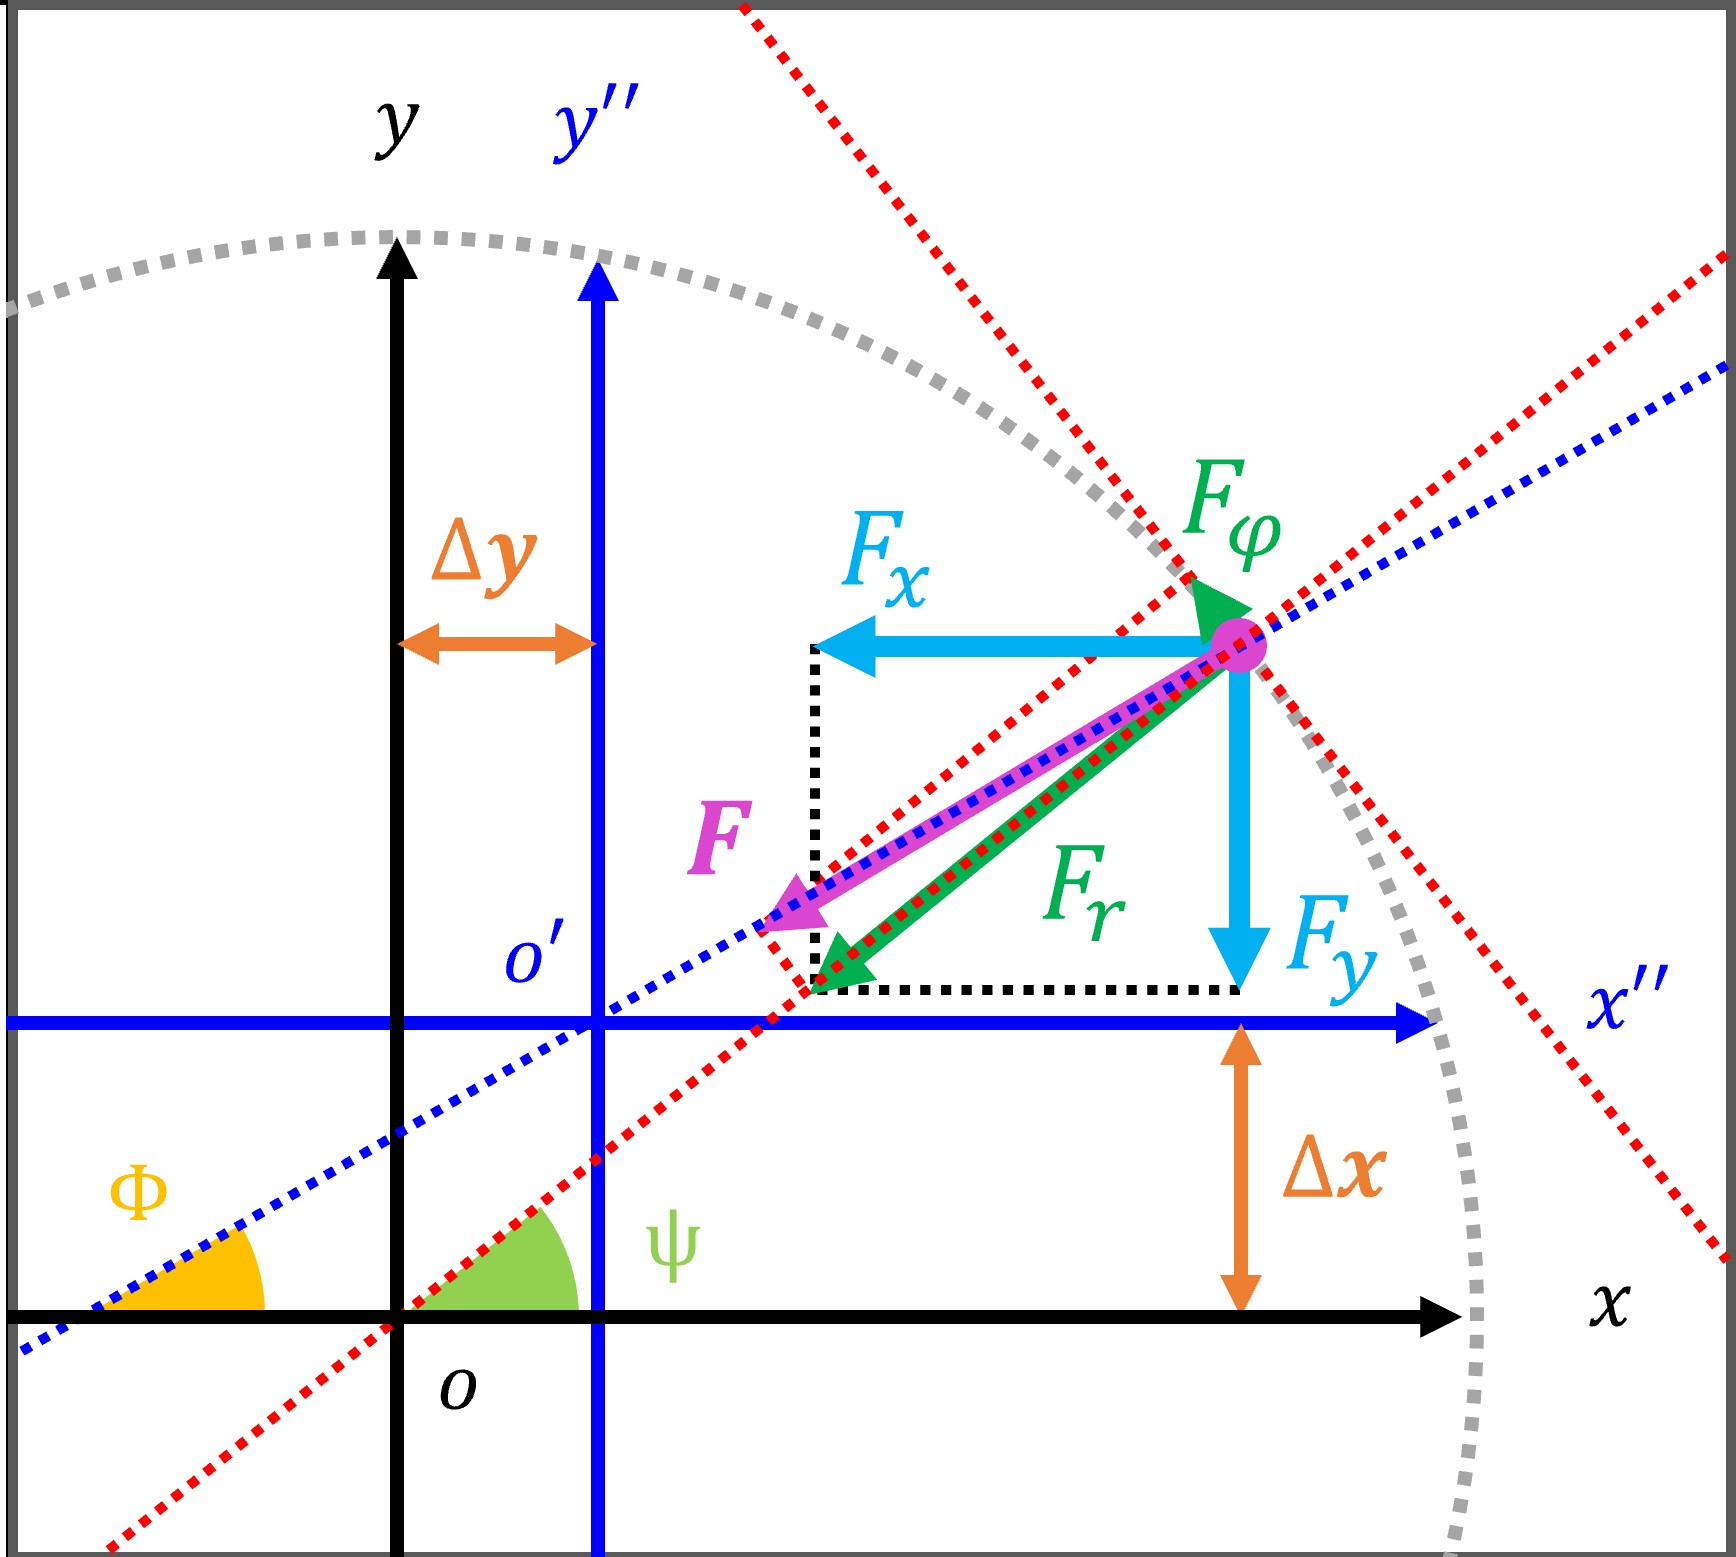
\includegraphics[width=80mm]{../images/image_6.png}
        \caption{}
    \end{center}
\end{figure}

\subsection{角度$\alpha$の算出}
はじめに,作用点と点$o'$を通る直線(青点線)と$x''$軸の角度を$\theta$,
作用点と点$o$を通る直線(赤点線)と$x$軸の角度を$\varphi$とする.
また,作用点と点$o'$を通る直線(青点線)と作用点と点$o$を通る直線(赤点線)の角度を$\alpha$とするとき,


\begin{itemize}
    \item [$\blacksquare$] \textgt{作用点と点$o'$を通る直線及び点$o$を通る直線の角度 $\alpha$}
          \begin{eqnarray*}
            \alpha = \varphi - \theta
          \end{eqnarray*}
\end{itemize}

ここで,供試体の半径を$r$として,正規座標系における作用点$F\left(x,y\right)$の座標は
角度$\varphi$を用いて以下のように表される.

\begin{itemize}
    \item [$\blacksquare$] \textgt{正規座標系における作用点$F\left(x,y\right)$の座標}
          \begin{eqnarray*}
            x &=& r \cos \varphi\\
            y &=& r \sin \varphi\\
          \end{eqnarray*}
\end{itemize}

このとき,校正装置の座標系において,作用点$F\left(x, y\right)$は
$\Delta x$,$Delta y$を用いて以下のように表される.

\begin{itemize}
    \item [$\blacksquare$] \textgt{校正装置の座標系における作用点$F\left(x'',y''\right)$の座標}
          \begin{eqnarray*}
            x'' &=& r \cos \varphi - \Delta x\\
            y'' &=& r \sin \varphi - \Delta y\\
          \end{eqnarray*}
\end{itemize}

これより,角度$\varphi$は以下のように求められる.

\begin{itemize}
    \item [$\blacksquare$] \textgt{作用点と点$o$を通る直線(赤点線)と$x$軸の角度を$\varphi$}
          \begin{eqnarray*}
            \varphi = \tan ^{-1} \left(\frac{y''}{x''}\right) 
            = \tan ^{-1} \left(\frac{ r \sin \varphi - \Delta y}{ r \cos \varphi - \Delta x}\right) 
          \end{eqnarray*}
\end{itemize}

\subsection{角度$\psi$の算出}

\begin{itemize}
    \item [$\blacksquare$] \textgt{実際の作用力の角度 $\psi$}
          \begin{eqnarray*}
            \phi = \theta + \left(-1\right) × \sin^{-1}\left(\frac{\Delta y \sin \theta - \Delta x \cos \theta}{r}\right)
          \end{eqnarray*}
\end{itemize}

\newpage

% \subsection{作用力の$F_r$,$F_\psi$への分解とトルク$T$の影響}

% 供試体に加わる作用力$F$は供試体表面の接線方向の力$F_\varphi$,
% またその法線方向の力$F_r$に分けて考えることができる.
% 算出した$\psi$を用いると,それぞれ以下のように求められる.

% \begin{itemize}
%     \item [$\blacksquare$] \textgt{接戦方向の力$F_\varphi$,接戦と法線方向の力$F_r$の算出}
%           \begin{eqnarray*}
%               F_\varphi &=& F \sin \psi \\
%               F_r &=& F \cos \psi
%           \end{eqnarray*}
% \end{itemize}

% 接戦方向成分$F_\varphi$について,供試体に対してトルク$T$として作用することとなる.

% \begin{itemize}
%     \item [$\blacksquare$] \textgt{供試体へ作用するトルク$T$}
%           \begin{eqnarray*}
%               T &=& F_\phi \cdot r\\
%               &=& F \sin \psi \cdot r
%           \end{eqnarray*}
% \end{itemize}

% ここで,このトルク$T$について,
% 作用力測定装置に対する影響は十分に小さいと考えられることから無視できる.

\section{テストデータの作成}
オフセットを考慮したテストデータを複数条件で作成し,
補正結果について比較した.

\begin{itemize}
    \item [$\blacksquare$] \textgt{$\Delta x = 5 [\mathrm{mm}]$,$\Delta y = 5 [\mathrm{mm}]$ のとき}
\end{itemize}

\begin{figure}[htbp]
    \footnotesize
    \begin{center}
        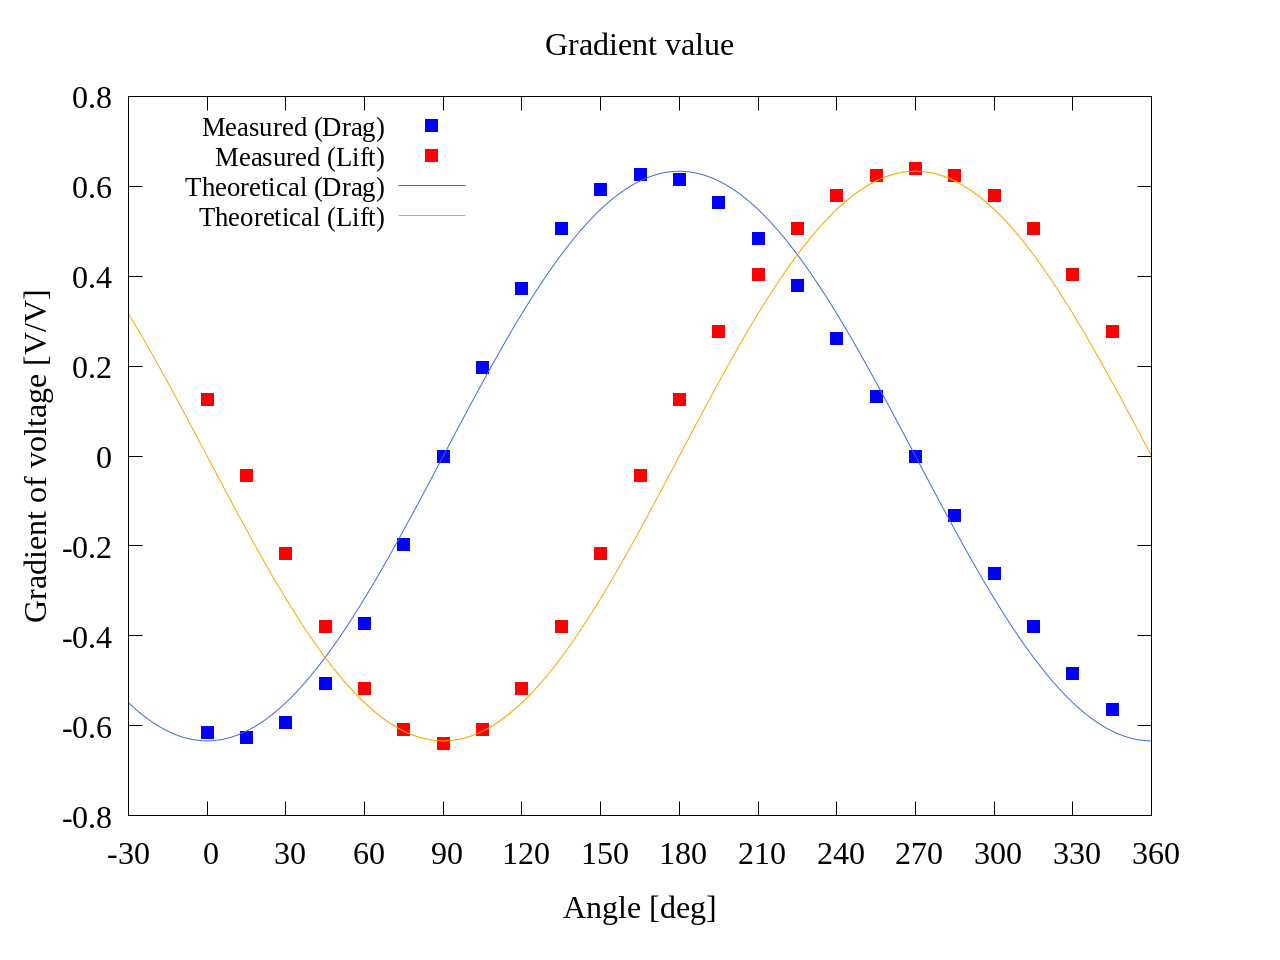
\includegraphics[width=86mm]{../graphes/offset_x=5_y=0/20/20_adjust-value.png}
        \caption{Summary of gradient voltage}
        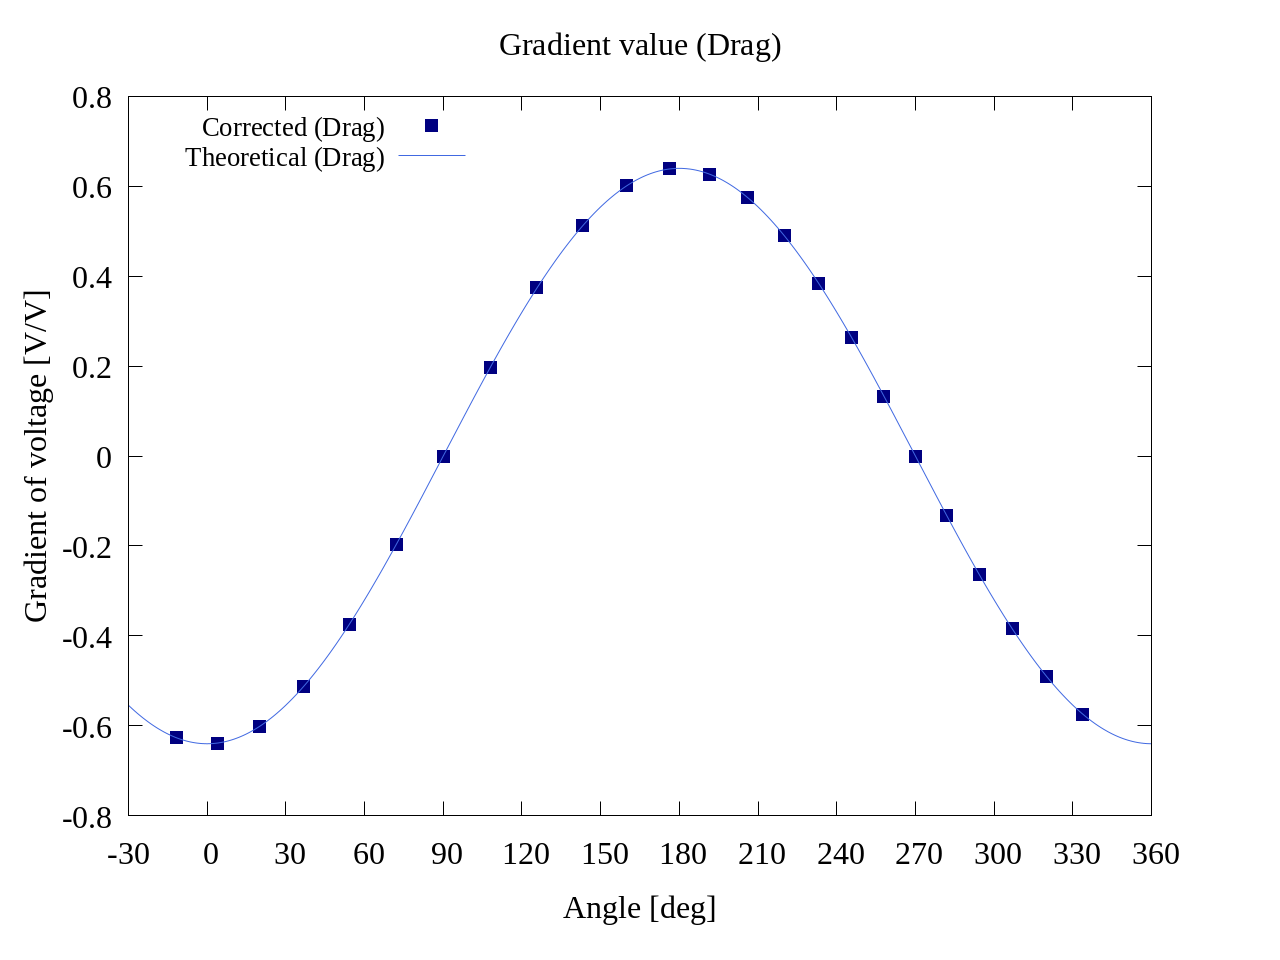
\includegraphics[width=86mm]{../graphes/offset_x=5_y=0/21/21-2_corrected_offset_drag.png}
        \caption{Corrected voltage (drag)}
        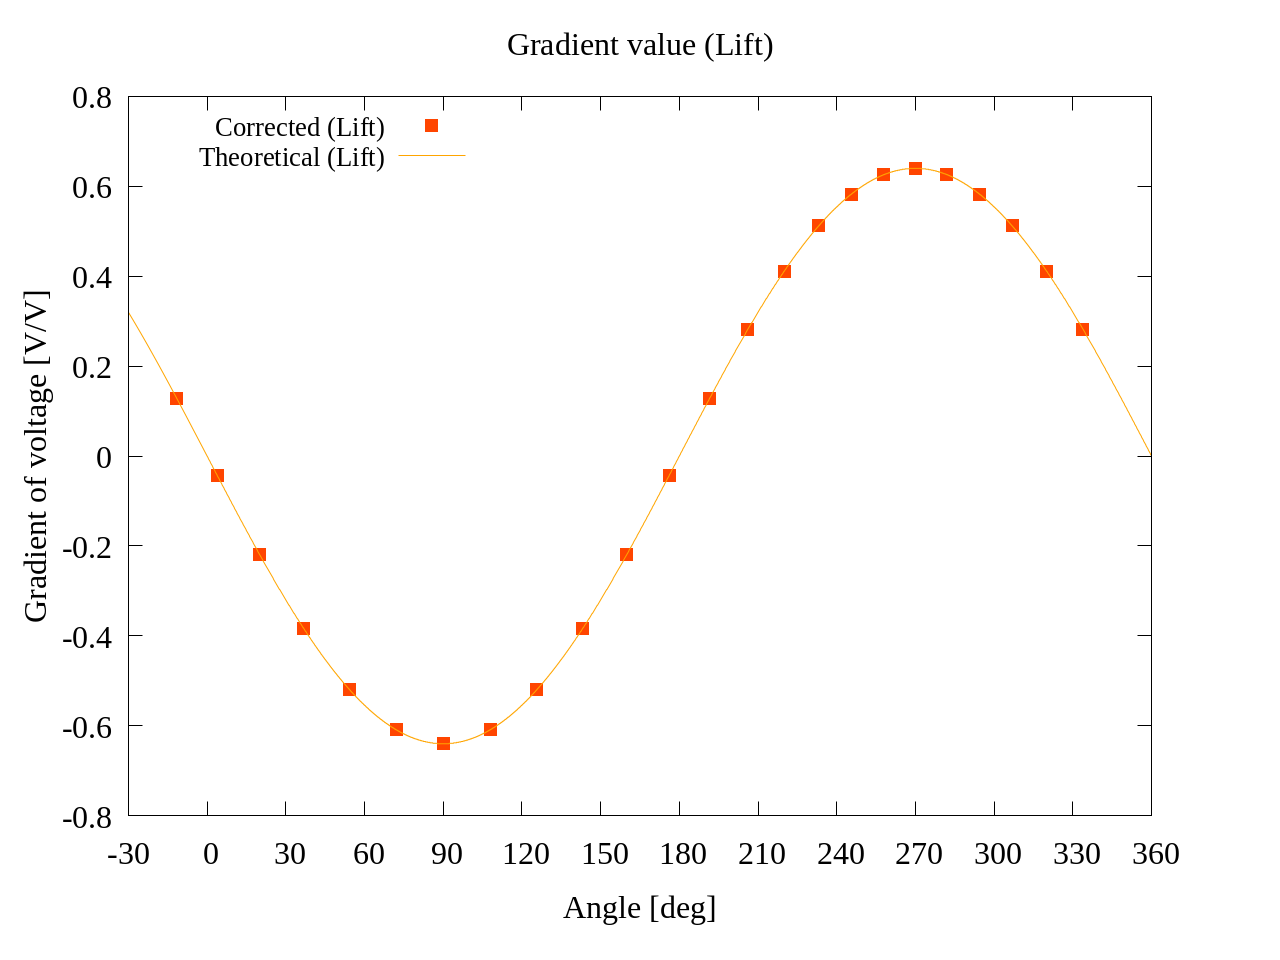
\includegraphics[width=86mm]{../graphes/offset_x=5_y=0/21/21-2_corrected_offset_lift.png}
        \caption{Corrected voltage (lift)}
    \end{center}
\end{figure}

\newpage

\begin{itemize}
    \item [$\blacksquare$] \textgt{$\Delta x = 5 [\mathrm{mm}]$,$\Delta y = 5 [\mathrm{mm}]$ のとき}
\end{itemize}

\begin{figure}[htbp]
    \footnotesize
    \begin{center}
        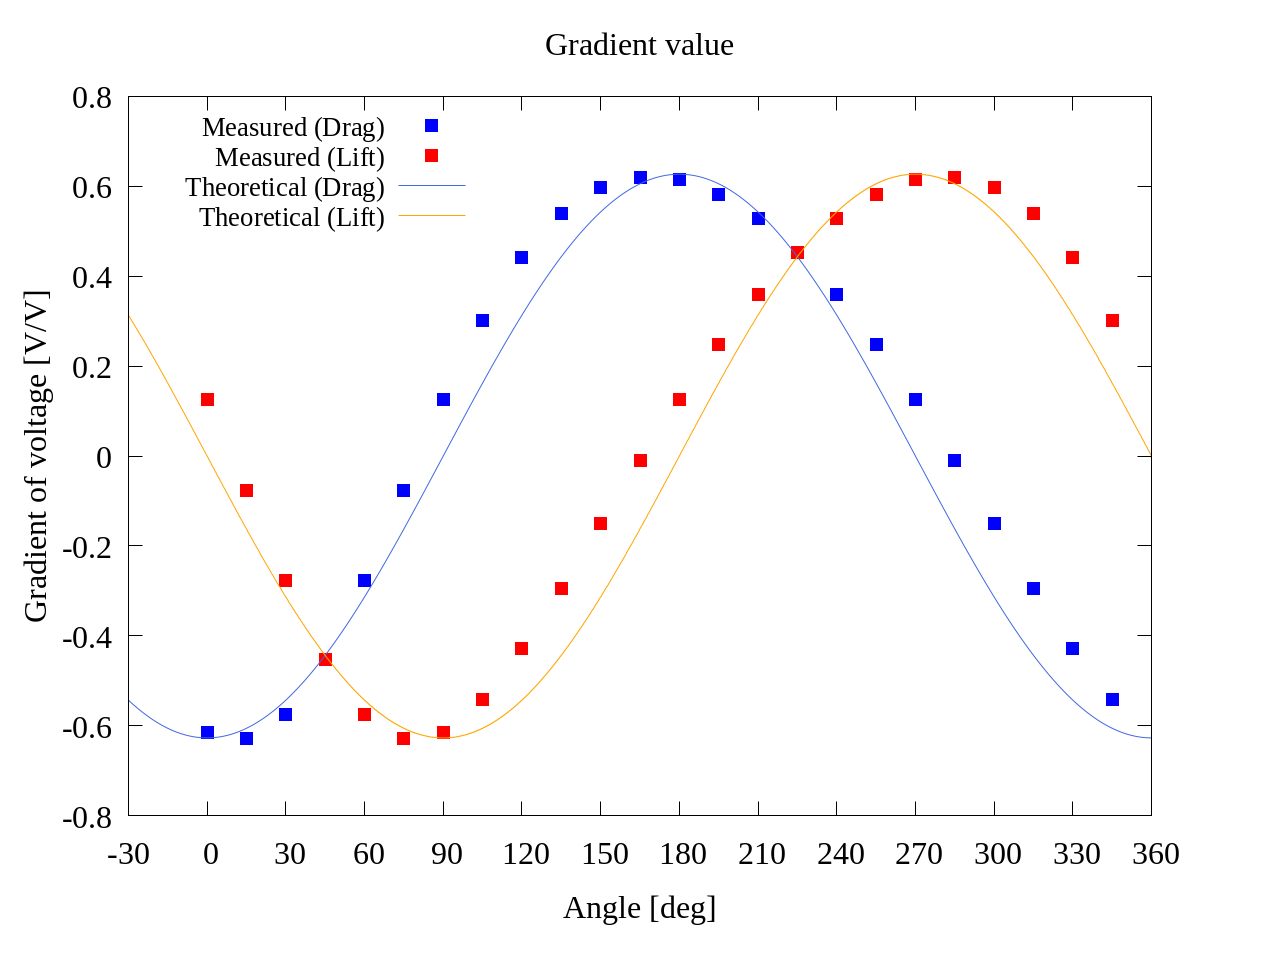
\includegraphics[width=86mm]{../graphes/offset_x=5_y=5/20/20_adjust-value.png}
        \caption{Summary of gradient voltage}
        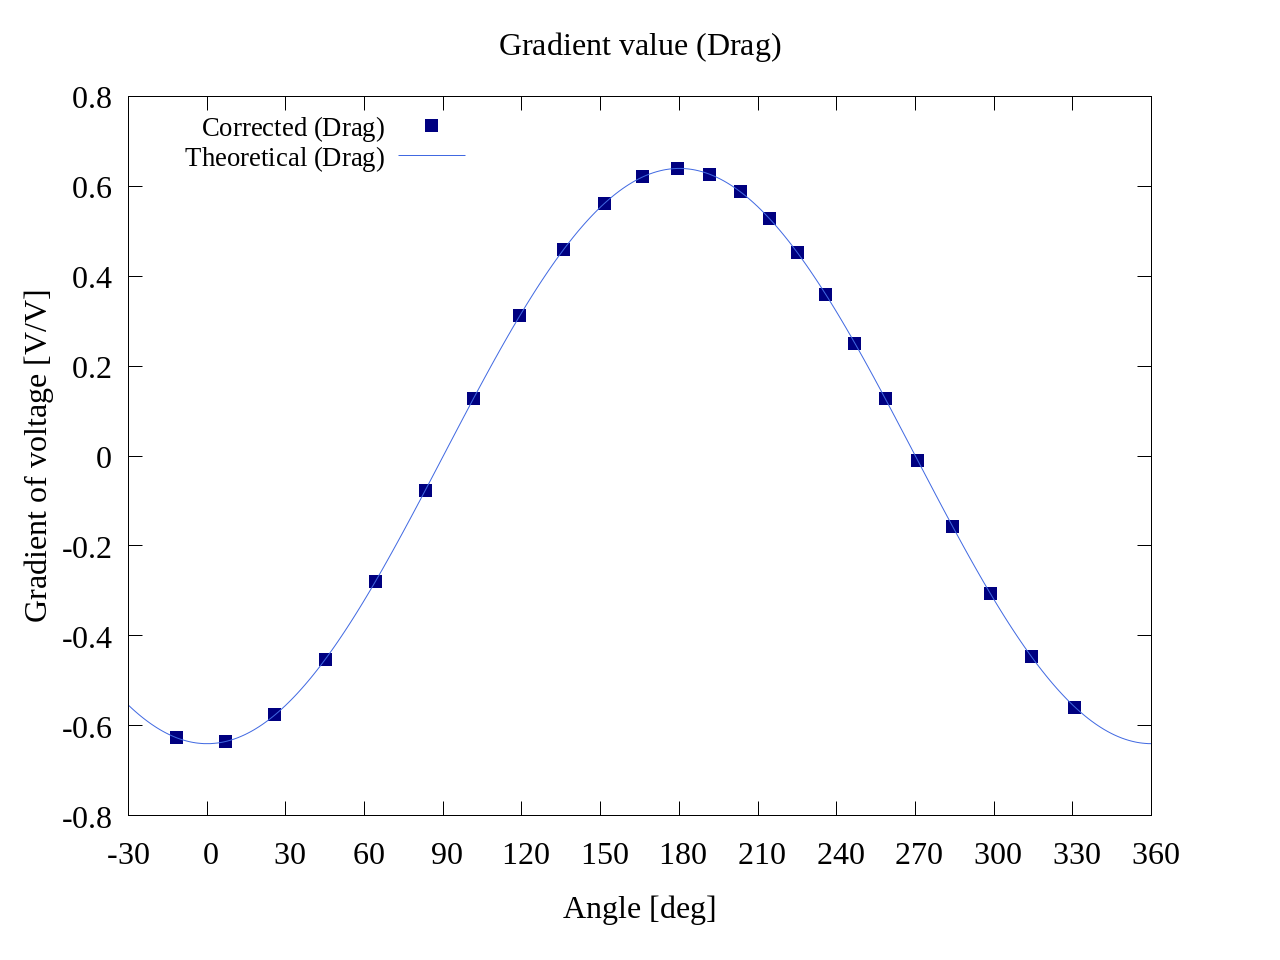
\includegraphics[width=86mm]{../graphes/offset_x=5_y=5/21/21-2_corrected_offset_drag.png}
        \caption{Corrected voltage (drag)}
        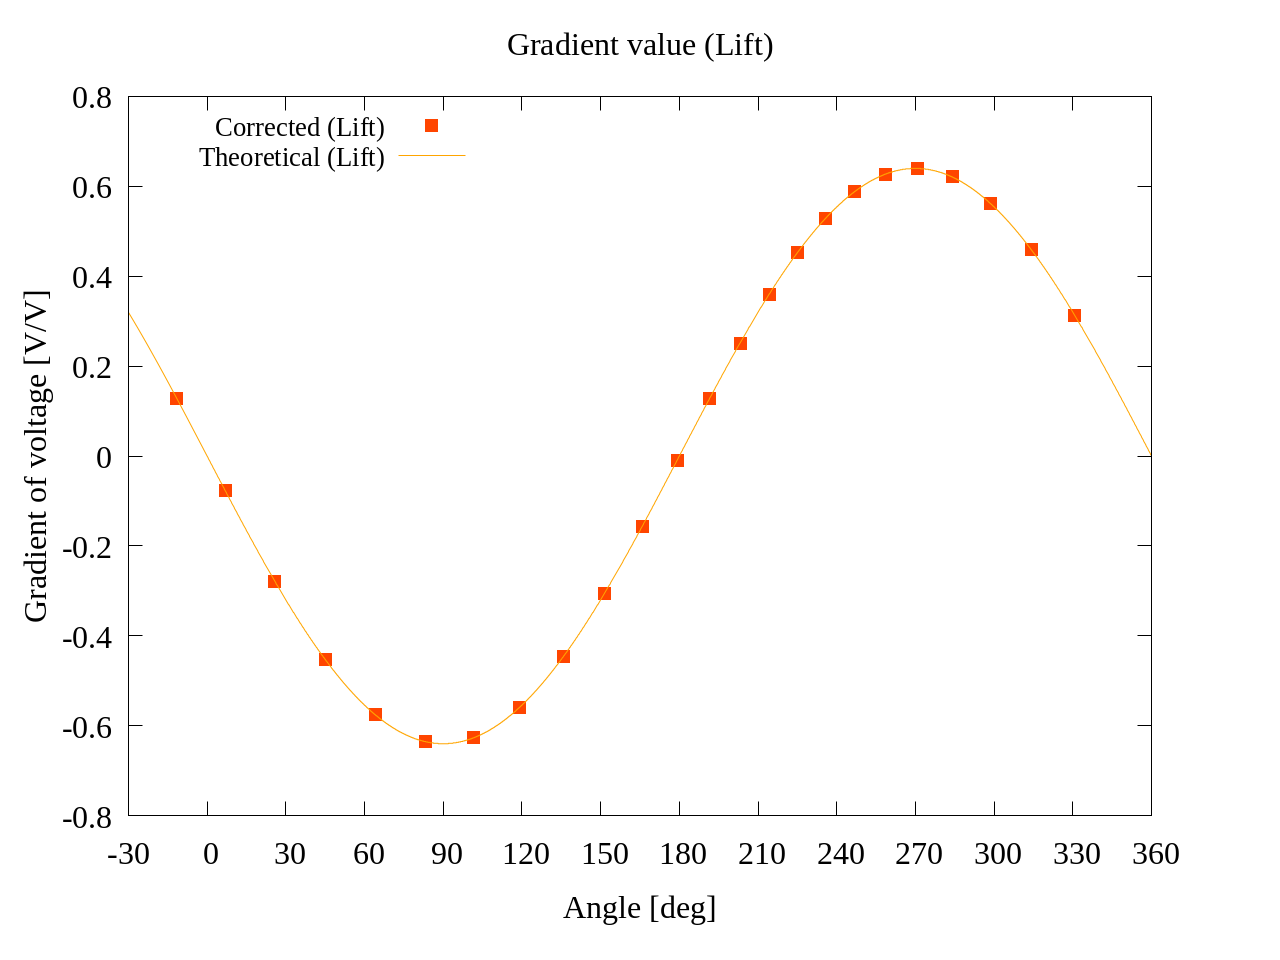
\includegraphics[width=86mm]{../graphes/offset_x=5_y=5/21/21-2_corrected_offset_lift.png}
        \caption{Corrected voltage (lift)}
    \end{center}
\end{figure}

\newpage

\begin{itemize}
    \item [$\blacksquare$] \textgt{$\Delta x = 10 [\mathrm{mm}]$,$\Delta y = 5 [\mathrm{mm}]$ のとき}
\end{itemize}

\begin{figure}[htbp]
    \footnotesize
    \begin{center}
        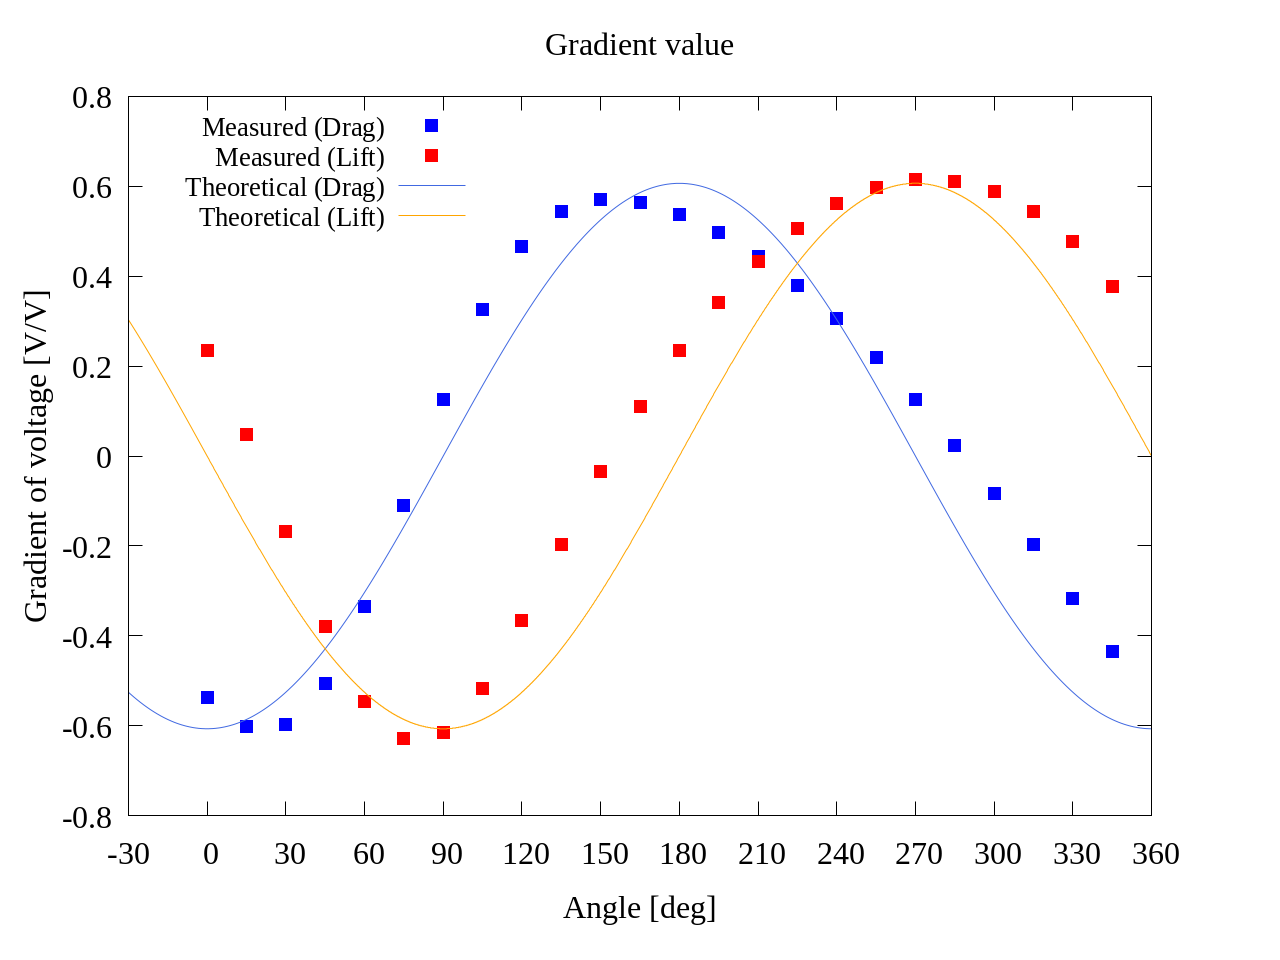
\includegraphics[width=86mm]{../graphes/offset_x=10_y=5/20/20_adjust-value.png}
        \caption{Summary of gradient voltage}
        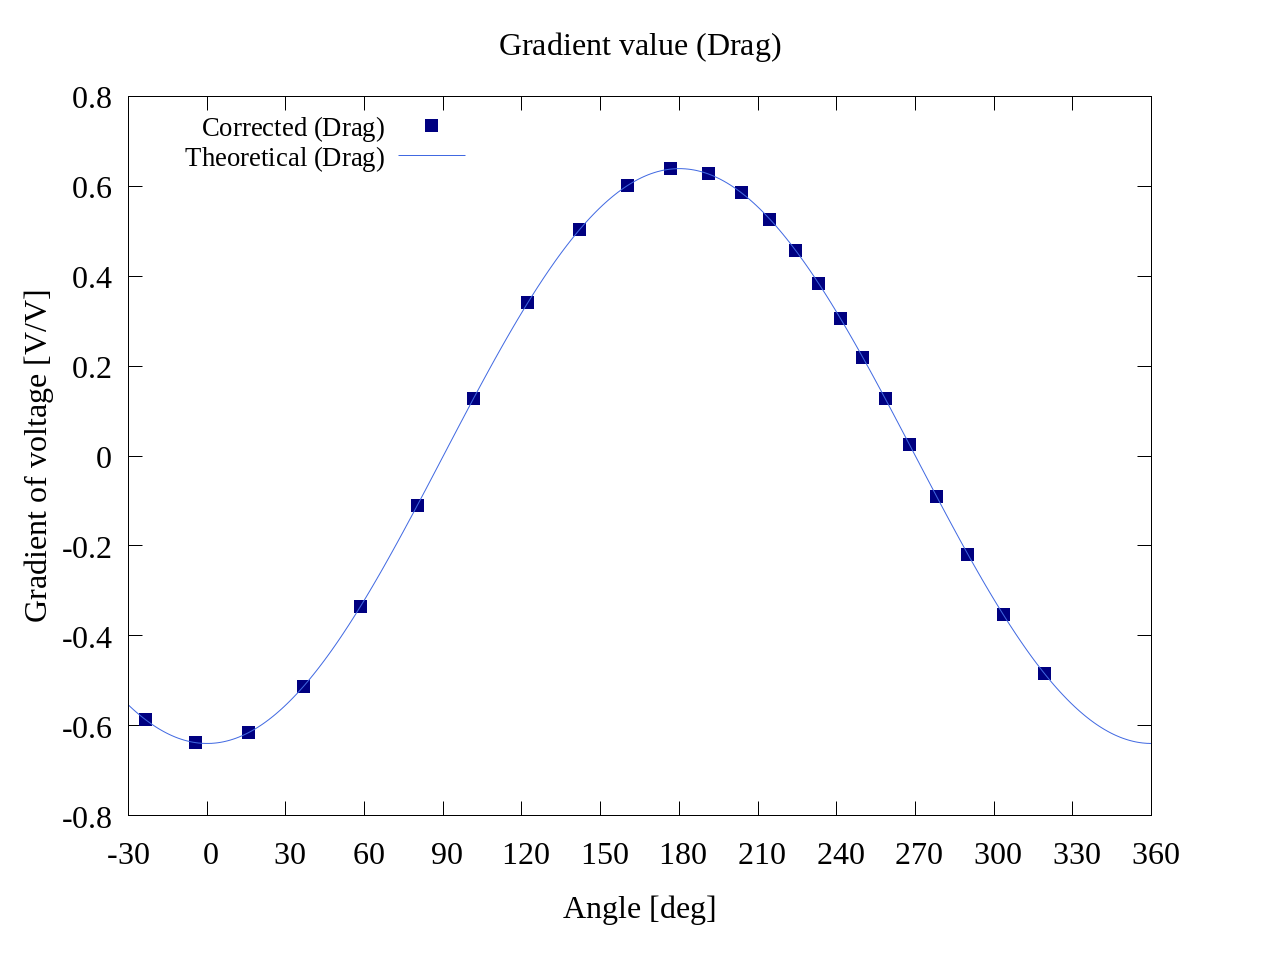
\includegraphics[width=86mm]{../graphes/offset_x=10_y=5/21/21-2_corrected_offset_drag.png}
        \caption{Corrected voltage (drag)}
        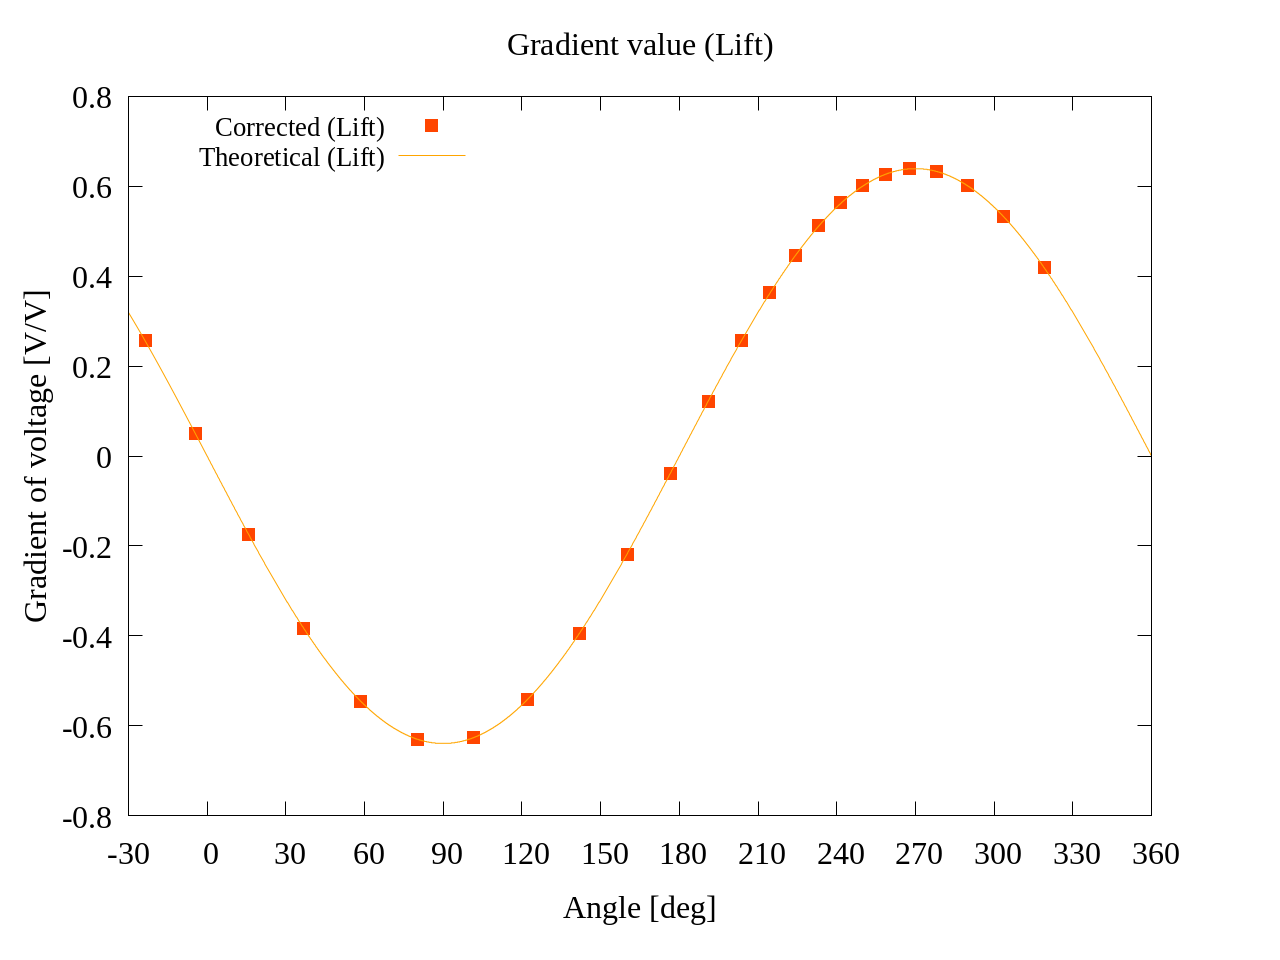
\includegraphics[width=86mm]{../graphes/offset_x=10_y=5/21/21-2_corrected_offset_lift.png}
        \caption{Corrected voltage (lift)}
    \end{center}
\end{figure}

\newpage

テストデータの補正適応結果から,理論曲線に重なるように補正することはできるが,
それぞれのデータの間隔が変化していることがわかる.
したがって,この補正結果に離散フーリエ変換を適用することは不可能であることがわかる.

\section{実験データとテストデータの比較}

変換理論を用いて,テストデータを作成した.
その結果を以下のFig.12~Fig.14に示す.
なお,テストデータ作成時にパラメータを以下のTable 1のように設定した.

\begin{table}[htbp]
    \begin{center}
        \caption{Simulation conditions}
        \begin{tabular}{|p{30mm}|p{20mm}|p{30mm}|}
            \hline
            \multicolumn{1}{|c|}{$x$軸の回転角}       & \multicolumn{1}{|c|}{$\theta_1$} & \multicolumn{1}{|c|}{7 [deg]}             \\ \hline
            \multicolumn{1}{|c|}{$y$軸の回転角}       & \multicolumn{1}{|c|}{$\theta_2$} & \multicolumn{1}{|c|}{5 [deg]}             \\ \hline
            \multicolumn{1}{|c|}{$x$軸のオフセット}   & \multicolumn{1}{|c|}{$\Delta x$} & \multicolumn{1}{|c|}{-1 [mm]}             \\ \hline
            \multicolumn{1}{|c|}{$y$軸のオフセット}   & \multicolumn{1}{|c|}{$\Delta y$} & \multicolumn{1}{|c|}{1.3 [mm]}             \\ \hline
        \end{tabular}
    \end{center}
\end{table}

ここで,それぞれの軸の回転角は,以前のプログラムからおおよその値を参照しており,
オフセット値については,以前の実験結果から概算したものである.
また,オフセットを考慮した際に算出される校正実験装置の押角$\phi$と
実際の作用力の角度$\psi$の関係性は以下のようになっている.

\begin{table}[htbp]
    \scalefont{0.9}
    \begin{center}
        \caption{True angle of acting force}
        \begin{tabular}{|p{20mm}|p{20mm}|p{20mm}|p{20mm}|}
            \hline
            \multicolumn{1}{|c|}{\textgt{$\phi$ [deg]}} & \multicolumn{1}{|c|}{\textgt{$\psi$ [deg]}}& \multicolumn{1}{|c|}{\textgt{$\phi$ [deg]}} & \multicolumn{1}{|c|}{\textgt{$\psi$ [deg]}}   \\ \hline
            \multicolumn{1}{|c|}{0}                     & \multicolumn{1}{|c|}{2.3}                  & \multicolumn{1}{|c|}{180}                   & \multicolumn{1}{|c|}{177.7}  \\ \hline
            \multicolumn{1}{|c|}{15}                    & \multicolumn{1}{|c|}{18.0}                 & \multicolumn{1}{|c|}{195}                   & \multicolumn{1}{|c|}{192.0}  \\ \hline
            \multicolumn{1}{|c|}{30}                    & \multicolumn{1}{|c|}{33.5}                 & \multicolumn{1}{|c|}{210}                   & \multicolumn{1}{|c|}{206.5}  \\ \hline
            \multicolumn{1}{|c|}{45}                    & \multicolumn{1}{|c|}{48.7}                 & \multicolumn{1}{|c|}{225}                   & \multicolumn{1}{|c|}{221.3}  \\ \hline
            \multicolumn{1}{|c|}{60}                    & \multicolumn{1}{|c|}{63.7}                 & \multicolumn{1}{|c|}{240}                   & \multicolumn{1}{|c|}{236.3}  \\ \hline
            \multicolumn{1}{|c|}{75}                    & \multicolumn{1}{|c|}{78.5}                 & \multicolumn{1}{|c|}{255}                   & \multicolumn{1}{|c|}{251.5}  \\ \hline
            \multicolumn{1}{|c|}{90}                    & \multicolumn{1}{|c|}{93.0}                 & \multicolumn{1}{|c|}{270}                   & \multicolumn{1}{|c|}{267.0}  \\ \hline
            \multicolumn{1}{|c|}{105}                   & \multicolumn{1}{|c|}{107.3}                & \multicolumn{1}{|c|}{285}                   & \multicolumn{1}{|c|}{282.7}  \\ \hline
            \multicolumn{1}{|c|}{120}                   & \multicolumn{1}{|c|}{121.4}                & \multicolumn{1}{|c|}{300}                   & \multicolumn{1}{|c|}{298.6}  \\ \hline
            \multicolumn{1}{|c|}{135}                   & \multicolumn{1}{|c|}{135.5}                & \multicolumn{1}{|c|}{315}                   & \multicolumn{1}{|c|}{314.5}  \\ \hline
            \multicolumn{1}{|c|}{150}                   & \multicolumn{1}{|c|}{149.5}                & \multicolumn{1}{|c|}{330}                   & \multicolumn{1}{|c|}{330.5}  \\ \hline
            \multicolumn{1}{|c|}{165}                   & \multicolumn{1}{|c|}{163.6}                & \multicolumn{1}{|c|}{345}                   & \multicolumn{1}{|c|}{346.4}  \\ \hline
        \end{tabular}
    \end{center}
\end{table}


\newpage

\subsection{テストデータ}

$\blacksquare$ \textgt{出力電圧の傾き(補正前)}

\begin{figure}[htbp]
    \footnotesize
    \begin{center}
        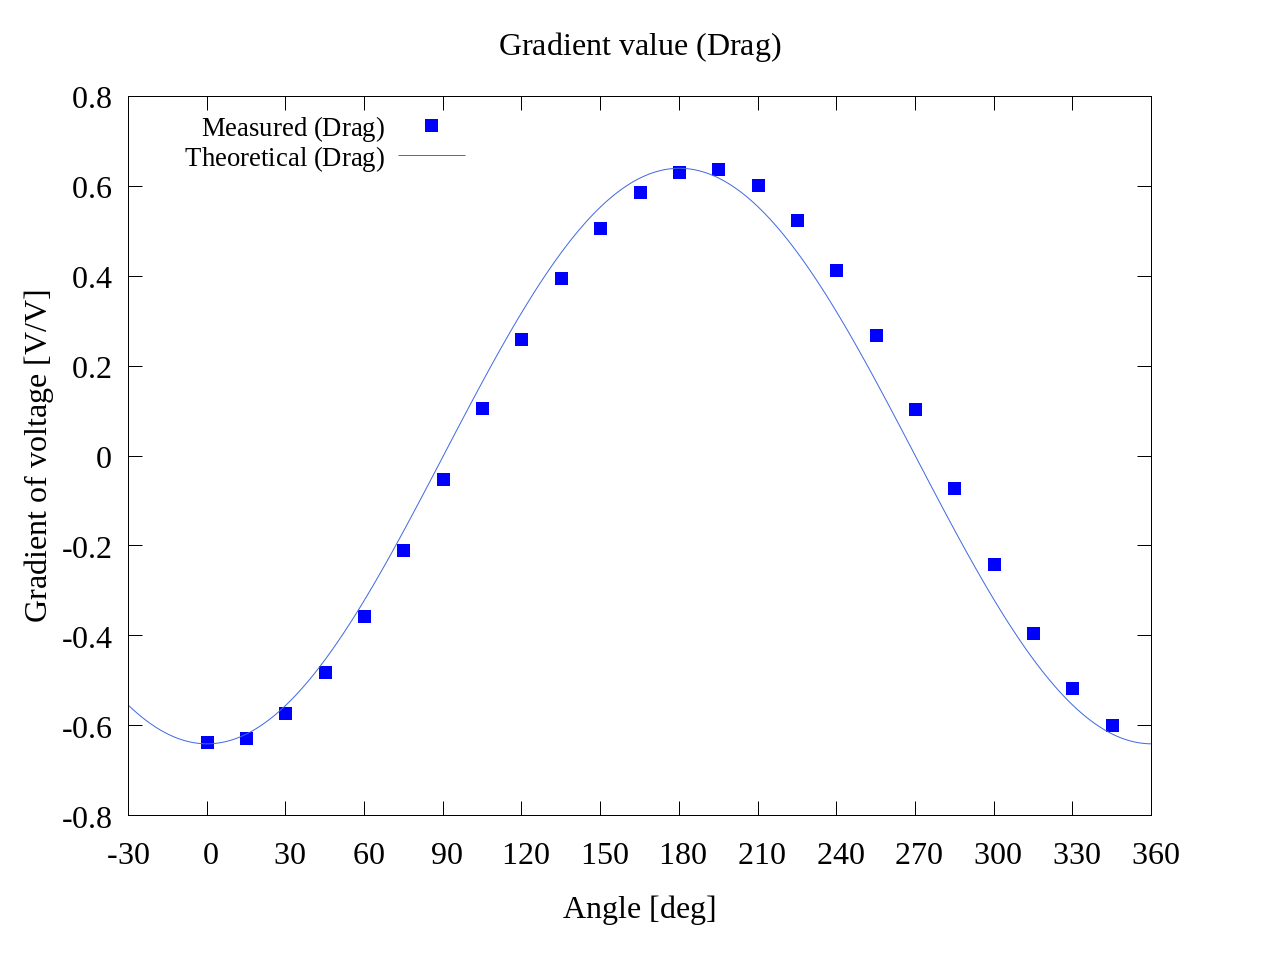
\includegraphics[width=86mm]{../graphes/simulation/21/21-1_summary_drag.png}
        \caption{Summary of gradient voltage (drag)}
        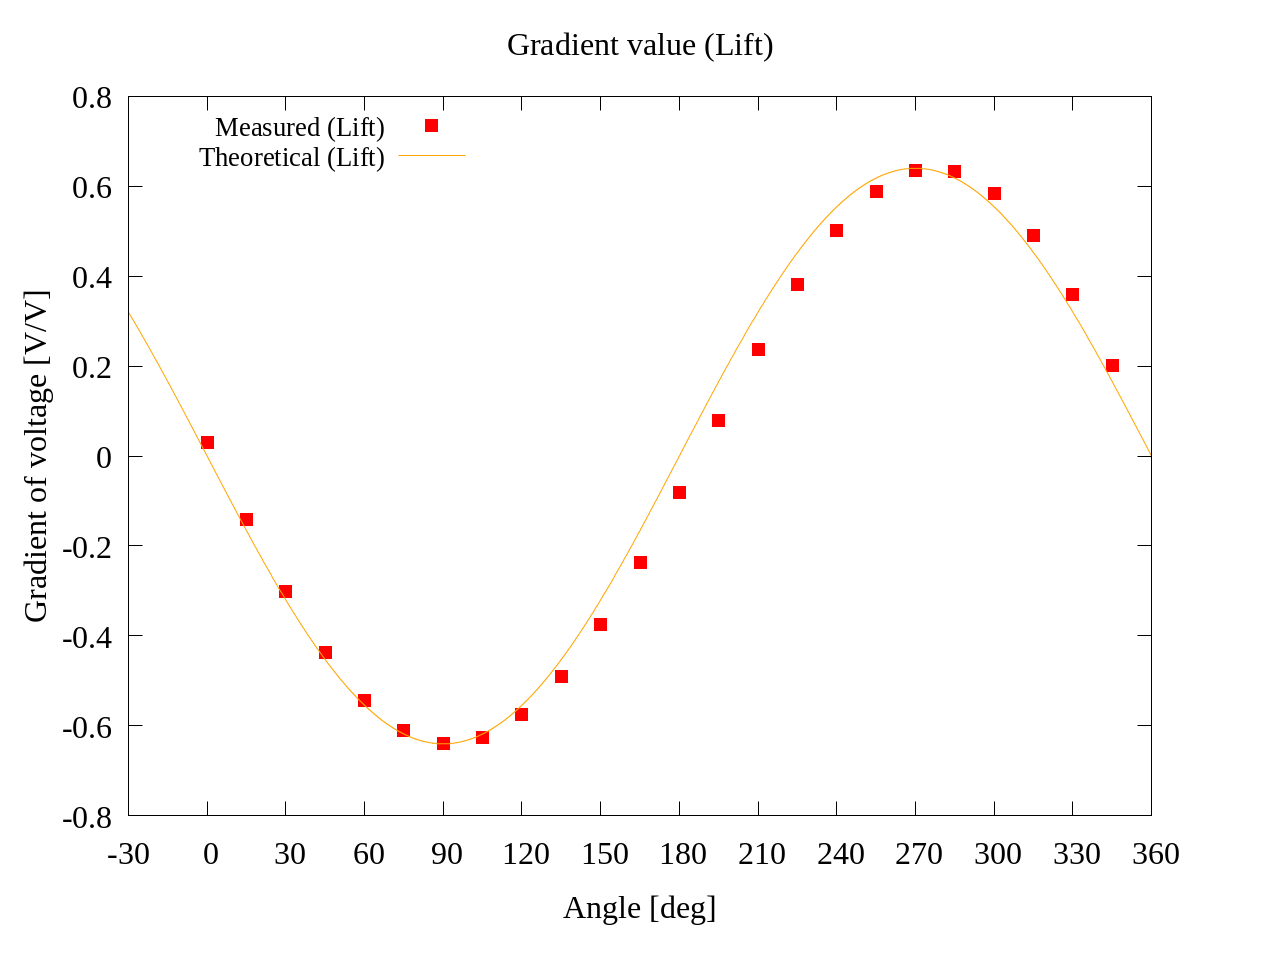
\includegraphics[width=86mm]{../graphes/simulation/21/21-1_summary_lift.png}
        \caption{Summary of gradient voltage (lift)}
    \end{center}
\end{figure}

$\blacksquare$ \textgt{正味出力電圧 (仮)}

\begin{figure}[htbp]
    \footnotesize
    \begin{center}
        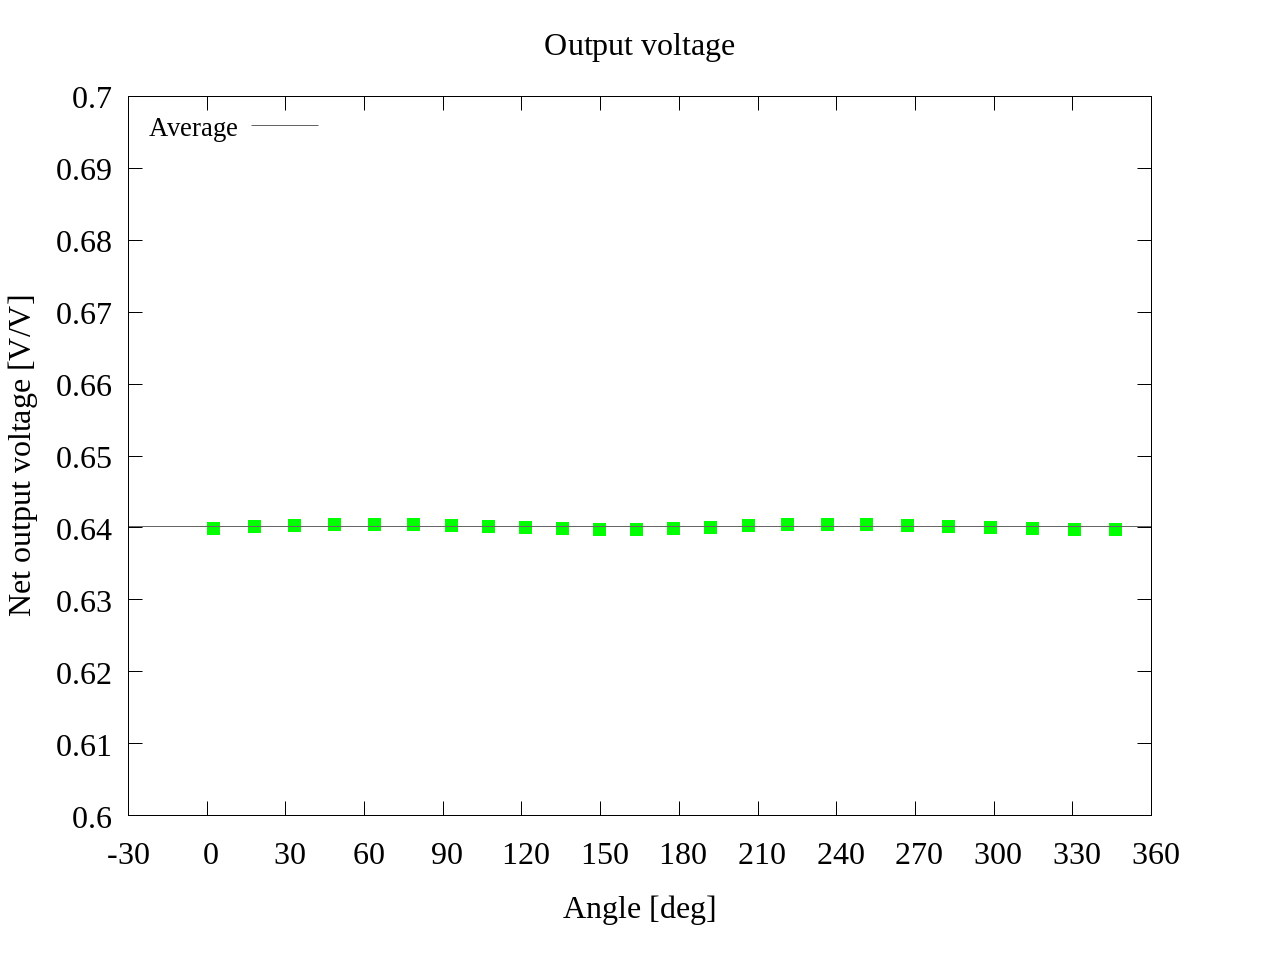
\includegraphics[width=86mm]{../graphes/simulation/09/09_summary-outputvoltage-net.png}
        \caption{Summary of net voltage (Corrected)}
    \end{center}
\end{figure}

\newpage

\subsection{実験結果}

$\blacksquare$ \textgt{出力電圧の傾き(補正前)}

\begin{figure}[htbp]
    \footnotesize
    \begin{center}
        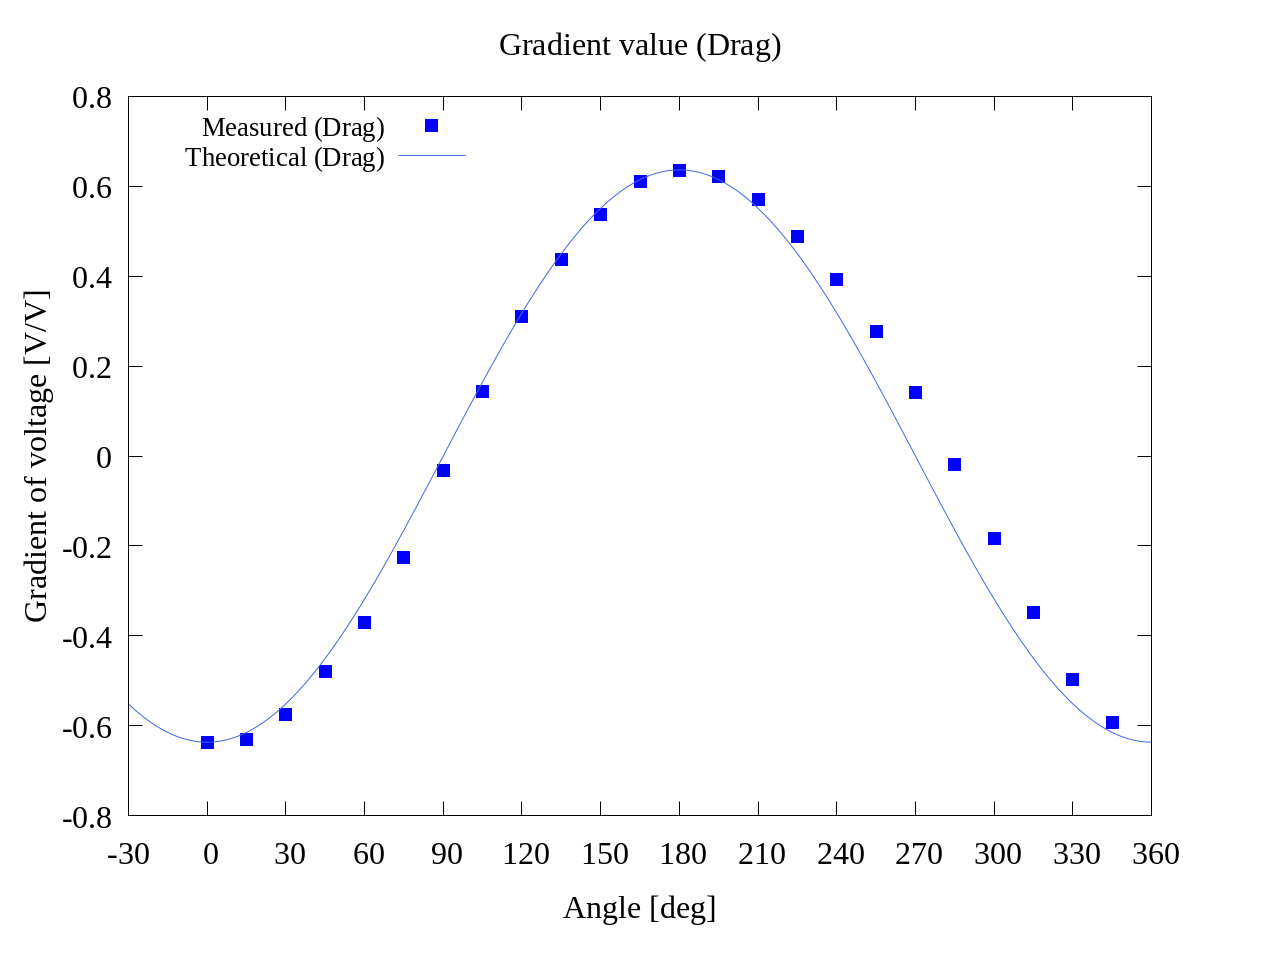
\includegraphics[width=86mm]{../graphes/1-ex/21/21-1_summary_drag.png}
        \caption{Summary of gradient voltage (drag)}
        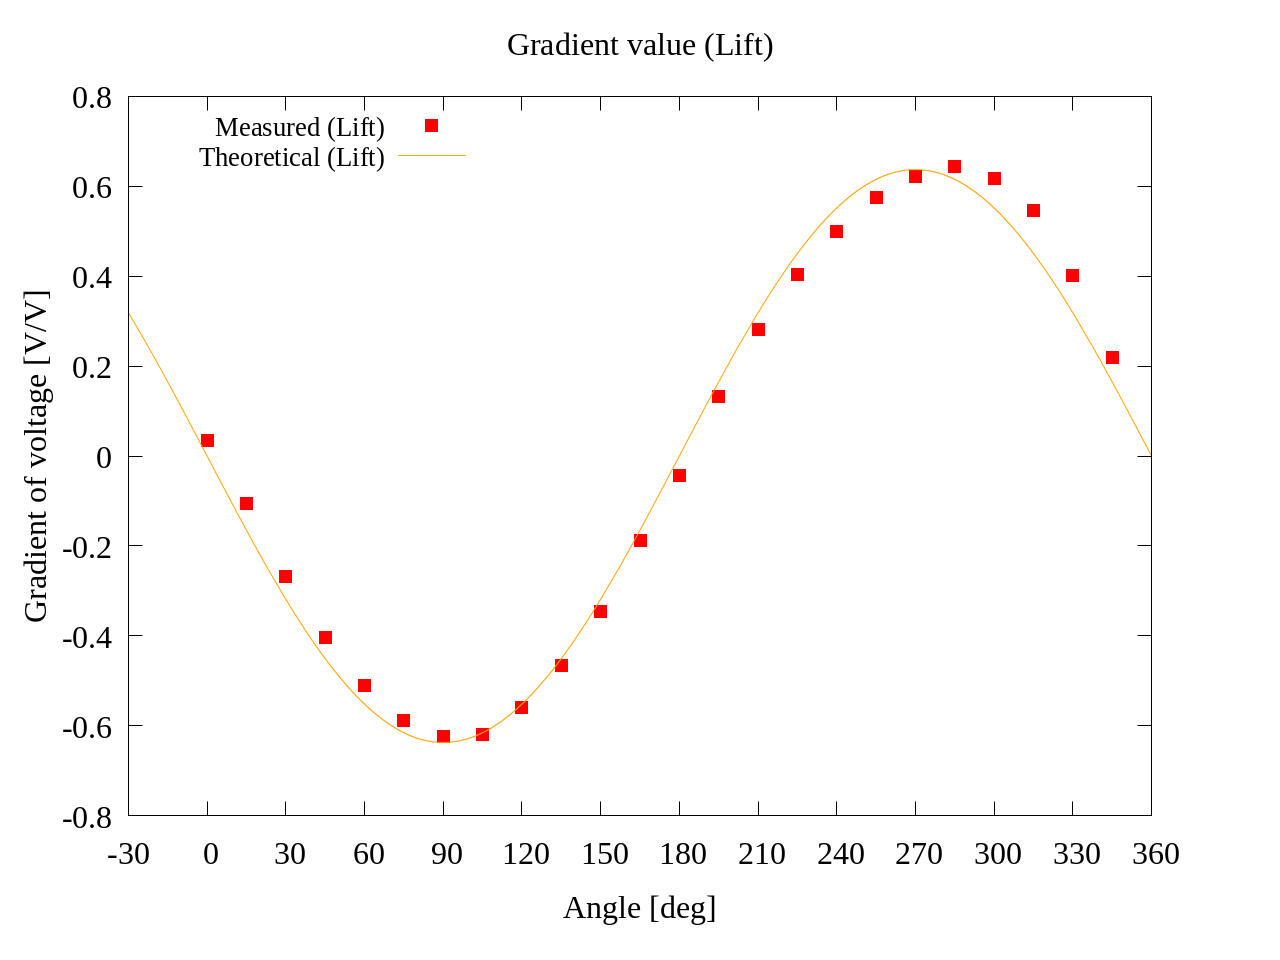
\includegraphics[width=86mm]{../graphes/1-ex/21/21-1_summary_lift.png}
        \caption{Summary of gradient voltage (lift)}
    \end{center}
\end{figure}

$\blacksquare$ \textgt{正味出力電圧(仮)}

\begin{figure}[htbp]
    \footnotesize
    \begin{center}
        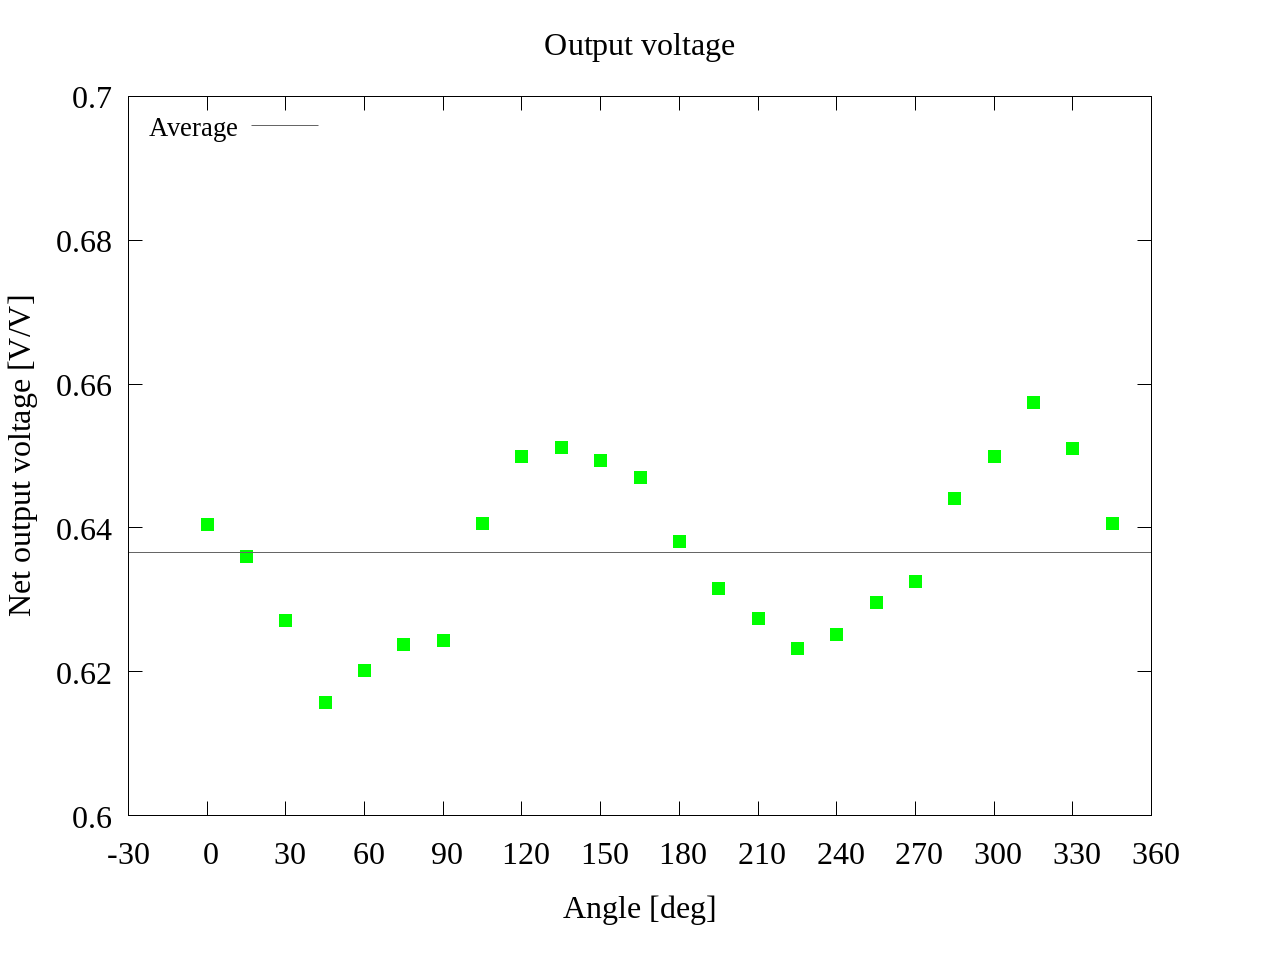
\includegraphics[width=86mm]{../graphes/1-ex/09/09_summary-outputvoltage-net.png}
        \caption{Summary of net voltage (Corrected)}
    \end{center}
\end{figure}

\newpage

$\blacksquare$ \textgt{正味出力電圧(仮) (補正前)}

\begin{figure}[htbp]
    \footnotesize
    \begin{center}
        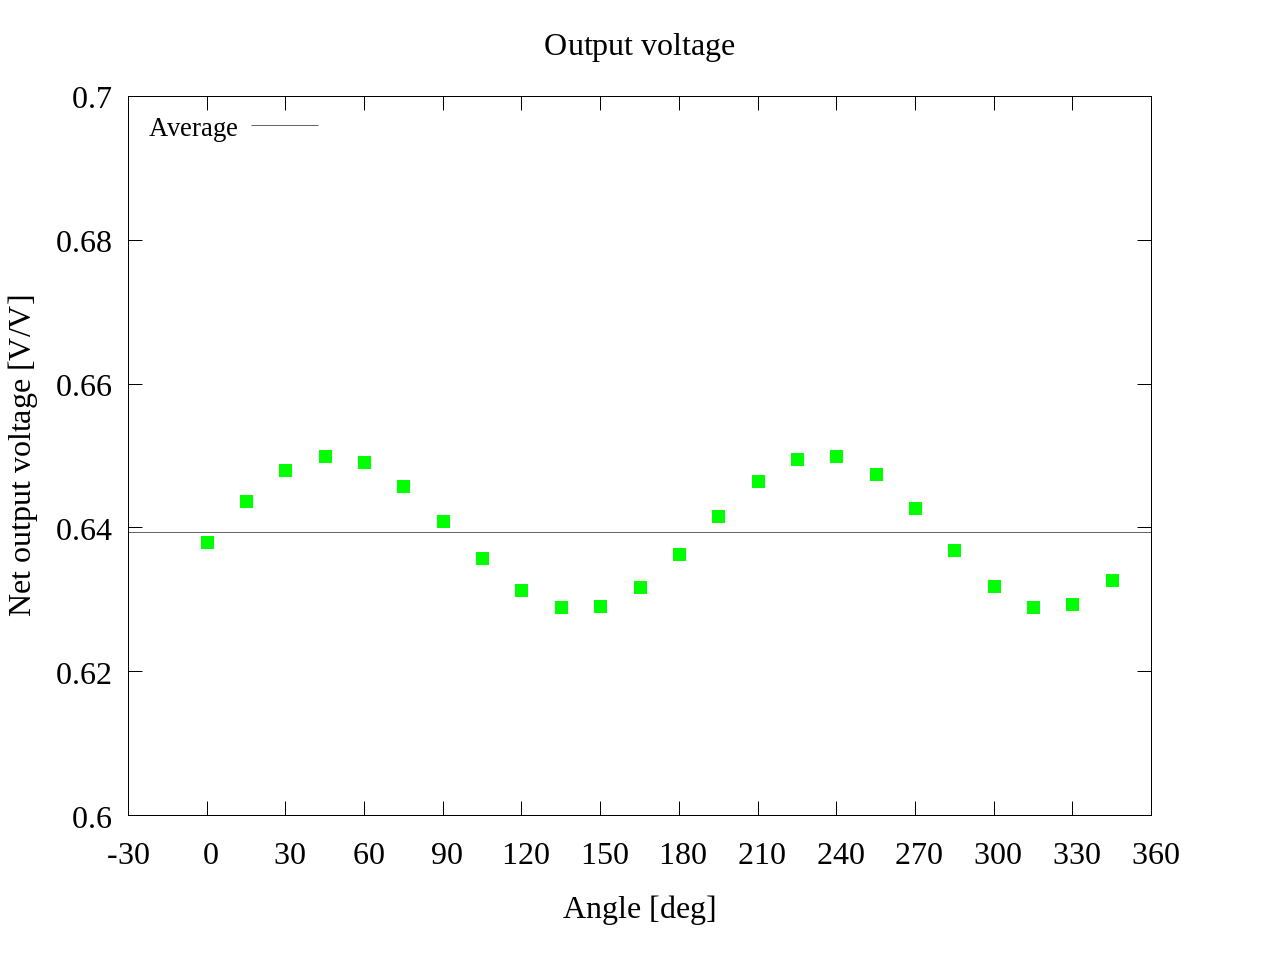
\includegraphics[width=86mm]{../graphes/simulation/05/05_summary-outputvoltage.png}
        \caption{Test data}
        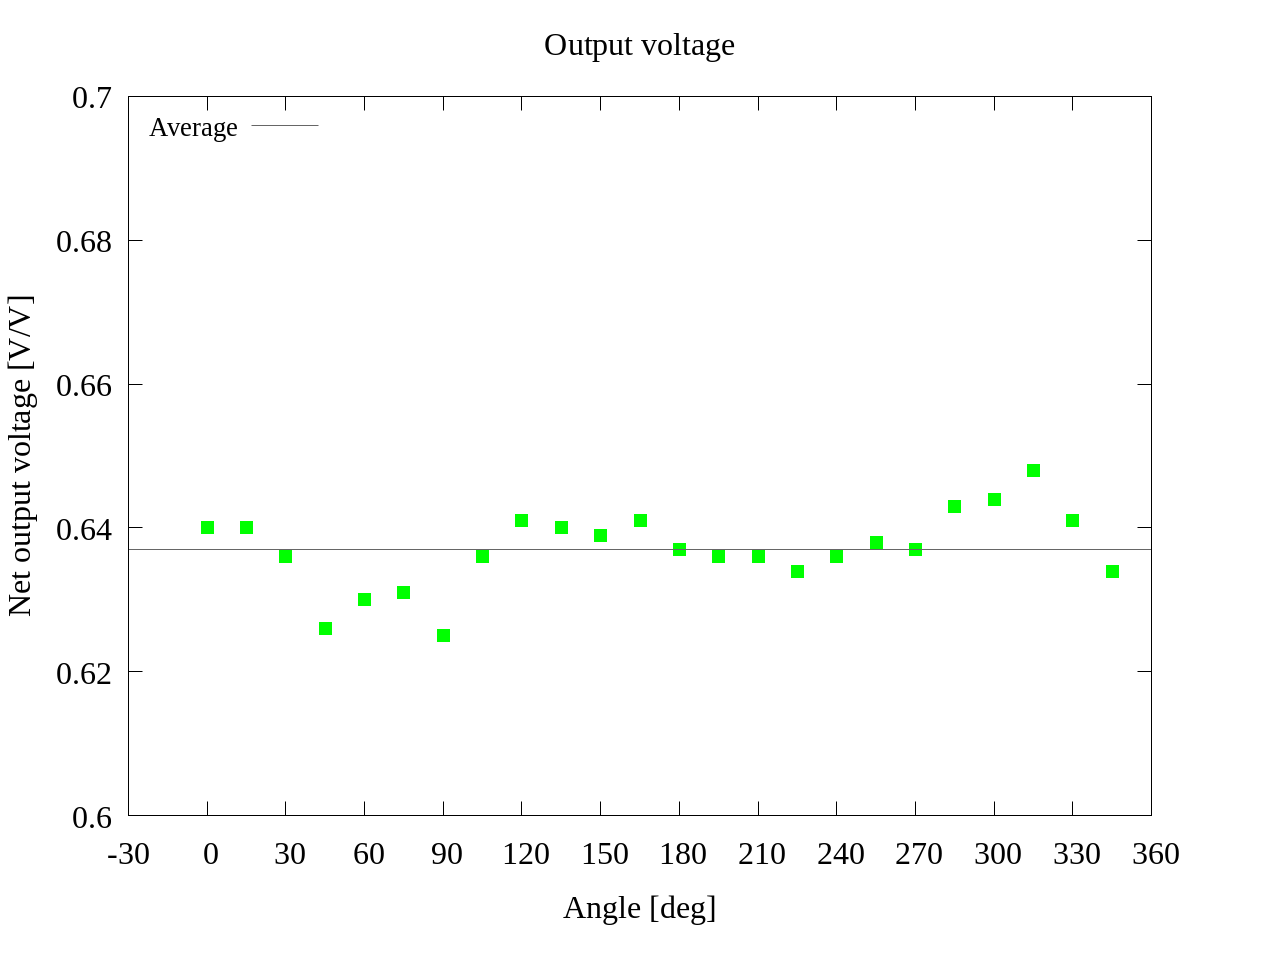
\includegraphics[width=86mm]{../graphes/1-ex/05/05_summary-outputvoltage.png}
        \caption{Experimental data}
    \end{center}
\end{figure}
\end{document}